% Supplementary material for the IEEE Transactions on Games submission (main_tog.tex); not counted in the page limit.
\documentclass[journal]{IEEEtran}
\usepackage{graphicx}
\graphicspath{{figures/}}
\renewcommand{\thefigure}{S\arabic{figure}}
\newcommand{\awr}{\textsc{ActiveWR}}

\begin{document}
\title{Supplementary Material: Winning Is Not Killing}
\author{Anonymous Author(s)}
\maketitle

\begin{figure*}[!h]
\centering
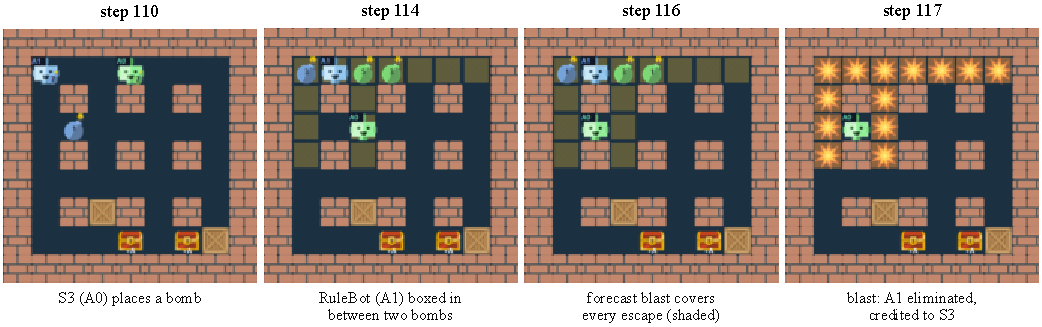
\includegraphics[width=\textwidth]{fig_gameplay.pdf}
\caption{Four frames of a real game: S3 (A0, green) against RuleBot (A1, blue) on validation board 21000. The number on a bomb is its fuse; shaded cells are the forecast blast area. S3's bombs at steps 110 and 112 box RuleBot in; the chain explosion at step 117 kills it and is credited to S3, so the game counts as an active win.}

\end{figure*}

\begin{figure*}[!h]
\centering
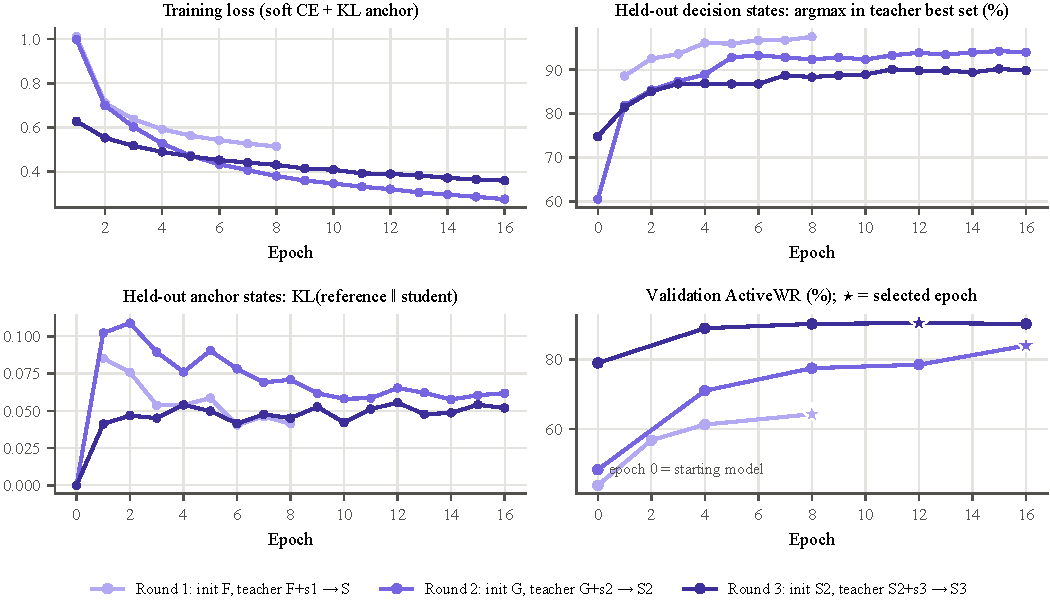
\includegraphics[width=\textwidth]{fig_distill_curves.pdf}
\caption{Distillation rounds. Top: training loss and share of held-out decision states where the student's argmax is in the teacher's best set. Bottom: KL from the starting policy on held-out anchors, and validation \awr{} (epoch 0 = starting model; stars = epochs selected before testing). Held-out sets differ between rounds.}

\end{figure*}

\begin{figure*}[!h]
\centering
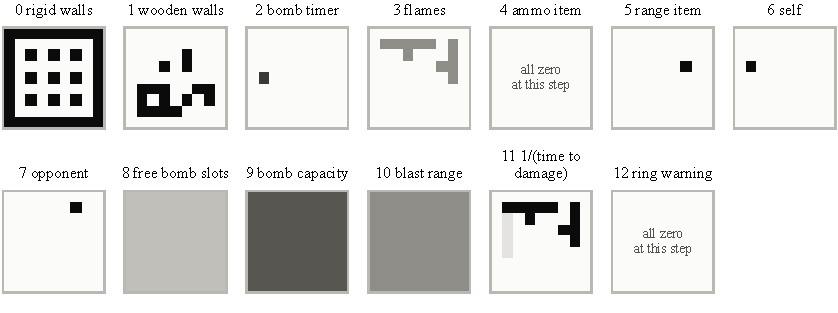
\includegraphics[width=\textwidth]{fig_observation.pdf}
\caption{The 13 observation planes for one agent (validation board 21007, step 26, RuleBot vs RuleBot; darker = larger). The agent has collected one ammo item (capacity 2 of 3) and has one bomb on the board, so one slot is free; a range item lies on the board. Planes marked ``all zero'' are empty at this step: no ammo item is visible, and the ring warning starts 40 steps before the first closure.}
\end{figure*}

\begin{figure*}[!h]
\centering
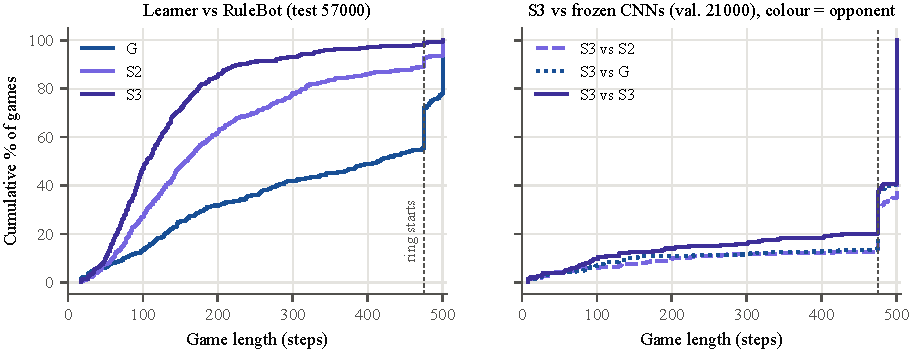
\includegraphics[width=\textwidth]{fig_episode_length.pdf}
\caption{Cumulative distribution of game length. Against RuleBot, stronger agents finish earlier (median 414, 158 and 105 steps for G, S2, S3; 22.25, 6.5 and 0.75\% reach the limit). Against frozen CNNs (right; colour = opponent), 59.5--65\% of S3's games reach 500 steps. Left: test block 57000; right: validation block 21000.}
\end{figure*}

\begin{figure*}[!h]
\centering
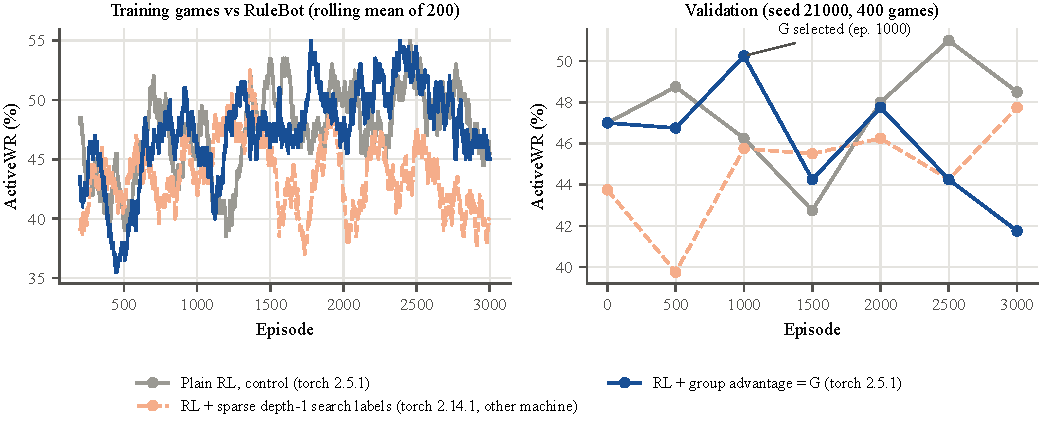
\includegraphics[width=\textwidth]{fig_training_curves.pdf}
\caption{RL from F (3{,}000 episodes per arm, one train seed). Left: rolling active win rate of training games against RuleBot. Right: validation active win rate every 500 episodes. The group-advantage arm peaked at episode 1000 (50.25) and became G; on the test block it was $+0.75$ over the control. The dashed arm ran on a second machine with another torch version, so its validation numbers are not comparable with the other two.}
\end{figure*}

\end{document}
